% !TeX root = ../index.tex
\documentclass[../index.tex]{subfiles}

\begin{document}
    \section{Wykład}
        \textbf{Galaktyka} to zbiorowisko gwiazd. Nasz układ słoneczny jest część galaktyki o nazwie \textbf{Droga Mleczna}, którą można obserwować na nocnym niebie. Jej jasność na niebie zależy od kierunku patrzenia – świadczy to o niecentralnym położeniu Słońca w galaktyce. Droga mleczna ma okrągły spłaszczony kształt (dysk lub elipsoida), jednak można w niej wyróżnić także ramiona (co najpierw zaobserwowano w innych galaktykach, znacznie później w naszej).\\
        Przeszkodą w identyfikacji ramion naszej galaktyki była silna koncentracja pyłu i gazu między gwiazdowego w płaszczyźnie dysku. Na pomoc przyszły obserwacje w zakresie podczerwienie oraz częstości radiowych. Typowe dla ramion spiralnych są koncentracje występowania wodoru międzygwiazdowego, które można identyfikować prowadząc obserwacje w linii wodoru neutralnego (przejście kwantowe wodoru polegające na zmianie kierunku spinu elektronu na powłoce podstawowej). Systematyczne skanowanie różnych kierunków w pasie Drogi Mlecznej daje szansę skonstruowania całościowego obrazu ramion spiralnych. Pierwsze próby był© mocno fragmentaryczne, ale wybór obłoków (H II) zjonizowane go wodoru, jako znaczników przebiegu ramion spiralnych poprawił otrzymany obraz. Obłoki H II różnią się od zwykłego wodoru międzygwiezdnego temperaturą ze względu na obecność pobliskich młodych gwiazd.\\
        W dalekiej podczerwieni zaobserwowano cztery główne ramiona wychodzą ze \textbf{zgrubienia centralnego} – elipsoidalnego centrum galaktyki. Ze względu na kształt zgrubienia centralnego, który przypomina poprzeczkę, nasza galaktyka nosi miano \textbf{galaktyki spiralnej z poprzeczką}.
        \begin{center}
            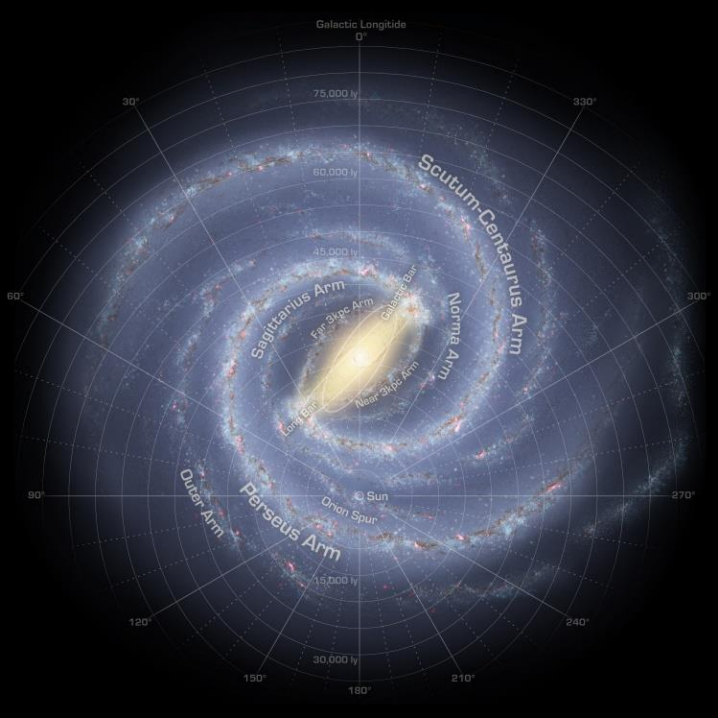
\includegraphics[width=9cm]{images/drogaMleczna.png}
        \end{center}
        Zaprezentowany obraz galaktyki nie jest kompletny. Oprócz gwiazd znajdujących się w płaszczyźnie dysku można zaobserwować nietypowe, bo ze znacznie niższą metalicznością (starsze) niż Słońce i większość gwiazd oraz z dużą prędkością względną. Zalicza się je tzw. \textbf{halo galaktycznego} lub do struktury pośredniej nazwanej \textbf{grubym dyskiem}. Charakteryzują się orbitami o różnym kącie nachylenia względem płaszczyzny dysku, w którym rotacja jest bardziej uporządkowana.
        \begin{center}
            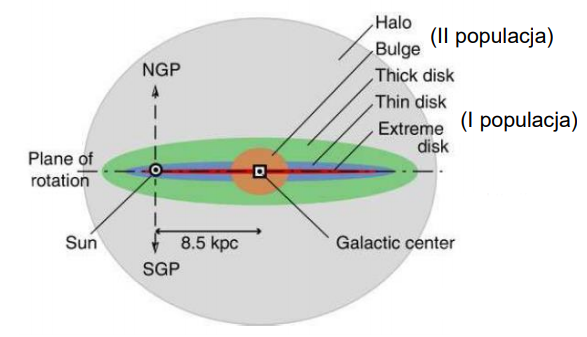
\includegraphics[width=13cm]{images/drogaMlecznaBudowa.png}
        \end{center}
        Powyżej można zobaczyć pełny obraz naszej galaktyki. Warto zwrócić uwagę, że przynależność do różnych składowych znajduje bezpośredni związek z wiekiem gwiazd.\\
        Wiek naszej galaktyki szacuje sie na kilkaset milionów lat mniej niż wiek wszechświata. Początkowa miała kształt sferycznie symetryczny i orbity gwiazd wówczas powstałych, które dziś należą do halo, odtwarzają go z grubsza. Obłoki materii, z których nie uformowały się wówczas gwiazdy, zaczęły wędrować do płaszczyzny prostopadłej względem osi rotacji. Za główną przyczynę tego procesu uważa się zderzenia między nimi, które następowały stosunkowo często (raz na kilkaset milionów lat) ze względu na ich duże rozmiary. Gwiazdy halo zachowały swoje oryginalne orbity ze względu na bardzo rzadkie zderzenie (raz na kilkanaście miliardów lat). w dalszej ewolucji procesy gwiazdotwórcze ograniczyły się tylko do dysku galaktycznego, bo tylko tam występował rozproszona materia. Dysk jest jaśniejszy od halom bo tylko w tym miejscu mogą świecić masywne, jasne i krótko żyjące gwiazdy. Dodatkowo koncentracja gwiazd w halo jest znacznie mniejsza.\\
        \textbf{Ramiona spiralne} są tworzone przez gwiazdy i obłoki materii międzygwiezdnej, których koncentracja jest wyraźnie większa niż w obszarach pomiędzy ramionami. Jednak przynależność do ramion nie jest czymś stałym, przeciwnie wszystkie obiekty obiegające centrum galaktyki znajdują się na przemiana w obrębie któregoś z ramion (najpierw na jednym, potem na drugim) albo poza nimi. Mechanizm istnienia ramion spiralnych opiera się na pojęciu \textbf{fal gęstościowych}. Oddziaływanie grawitacyjne koncentracji materii, jaką stanowią ramiona, powoduje, że każdy obiekt uczestniczący w rotacji prędzej tam dociera i wolniej go opuszcza (podobnie jak w korku ulicznym – auta zbliżają się do niego z dużą prędkością, ale w korku poruszają się znacznie wolniej). Ramiona najprawdopodobniej ukształtowały się w wyniku bliskiego kontaktu z innym zbiorowiskiem gwiazd.\\
        W galaktykach można wyróżnić \textbf{gromady gwiazdowe} – zgrupowania gwiazd, które wspólnie powstały i nadal zachowują grawitacyjną spoistość. Wyróżnia się dwa podstawowe rodzaje:
        \begin{itemize}
            \item \textbf{Gromady otwarte} – są mniej liczne (od 100 do 10 000) gwiazd, mają słabszą koncentracje gwiazd i istnieją krótko (do 1 mld. lat). Przykładem takiej gromady są plejady.
            \item \textbf{Gromady kuliste} – są bardziej liczne (od \(10^{5}\) do \(10^{7}\)), mają sferycznie symetryczne rozmieszczenie składników z rosnącą koncentracją w stronę centrum i mogą mieć 10 mld., a nawet więcej lat. Przykładem jest \(\omega\) Centauri. Niektóre z tych gromad powstały w początkowych stadiach wszechświata.
        \end{itemize}
        Obecność gwiazdy w gromadzie ułatwia określenie jej wieku. Zgodnie z teorią ewolucji młode gwiazdy układają się na diagramie H-R w zależności od masy na ciągu głównym. Im gwiazda ma większą masę tym szybciej opuszcza ciąg główny. Oznacza to, że w przypadku każdej gromady istnieje punkt na ciągu głównym, powyżej którego nie ma już żadnej gwiazdy. Wystarczy wiedzieć ile czasu potrzeba na całkowite wypalenie wodoru w centrum gwiazdy o masie odpowiadającej temu punktowi, żeby określić wiek gromady.\\
        Badania układu ramion spiralnych Drogi Mlecznej skutkowało określeniem jej \textbf{krzywej rotacji} – zależność prędkości obiegu wokół centrum galaktyki w zależności od odległości od tegoż centrum. Zależność ta nie przypomina ani rotacji ciałą sztywnego ani zależność z jaką planety okrążają Słońce w naszym układzie. Szczególny kłopot w interpretacji przynosi wysoka wartość prędkości rotacji na odległościach powyżej trzech kiloparseków. Podobne anomalne zachowanie wykazują też inne galaktyki. Ta zależność oznacza, że mamy do czynienia z czymś, czego natury jeszcze nie znamy – \textbf{ciemną materią}. Brane pod uwagę są różne wytłumaczenia tego zjawiska, między innymi neutrina i masywne, słabo oddziałujące cząstki (WIMP). Według różnych szacunków ciemnej materii jest tyle samo co materii barionowej (zwykłej) – w szacunkach tyczących się obrotu galaktyki lub nawet 5-6 razy więcej – gdy uwzględnia się oddziaływania między galaktykami.\\
        \textbf{Centrum galaktyki} znajduje się 8.54 kpc od nas, w gwiazdozbiorze Strzelca. Największą emisje wykazuje źródło Saggitarius A, a jego najbardziej zwartą część, oznaczaną \textbf{Sgr A\(^{*}\)} utożsamiana jest z \textbf{supermasywną czarną dziurą} o masie 4.3 milionów mas Słońca.
\end{document}